% Drawing 74/04-14 -- folder 74, batch 04, archive page 77 (PDF page 78).
% Transcription: à côté, un schéma : $t_1$, $t_2$, $t_0$ en colonne à gauche, $\alpha$, $\beta$, $\gamma$ en colonne à droite ; des traits joignent $t_1$ et $t_2$ à chacun de $\alpha$, $\beta$, $\gamma$ ; $t_1$ et $t_2$ sont entourés d'un ovale, une croix suit $t_0$, et un long trait presque vertical traverse le tout.
% Kind: bipartite scheme (t_1, t_2, t_0 against alpha, beta, gamma). Method 2 (schematic redraw from the facsimile). Status: partial.
% Notes: Right part of the same crop as 04-13. The letters t_1, t_2, t_0 in a column and alpha, beta, gamma in a column; pencil lines from t_1 and from t_2 to each of alpha, beta, gamma, leaving from one computed point beside each letter; an oval round t_1 and t_2; a cross after t_0; a long, nearly vertical pencil stroke across the whole scheme, drawn as on the page (it may be a strike or a separation: the table of couples (t_i, alpha) ... that follows on the page is not struck). Still differs: the pencil lines are faint and tangled, the six joins are a reading; no line from t_0 is seen. Id 04-14: existing ids are not renumbered. Redrawn 2026-11-12 (issue 128): to check again.
% Coordinates: 1 unit = 1 mm = 1/100 of the crop width (bbox in page fractions: [0.15, 0.085, 0.36, 0.16]).
% Redrawn by Claude (claude-fable-5-2), issue #128, 2026-11-12; not checked by a human; not compiled (no TeX in the session).
% Rights: reproduces part of the work -- behind RENDER_TRANSCRIPTS, never published by itself.
\documentclass[tikz,border=3pt]{standalone}
\usepackage{amsmath,amssymb}
\usetikzlibrary{patterns,arrows.meta}
\tikzset{pencil/.style={black!45}, struck/.style={black!35}, mpt/.style={circle,draw,inner sep=1.3pt}, pt/.style={circle,fill,inner sep=0.9pt}, opt/.style={circle,draw,fill=white,inner sep=1.1pt}}
\begin{document}
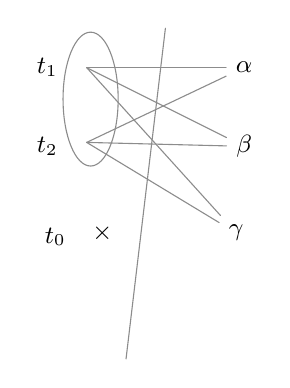
\begin{tikzpicture}[x=1mm,y=1mm,line cap=round,line join=round,font=\small]
\node (t1) at (65,-5) {\small $t_1$};
\node (t2) at (65,-15) {\small $t_2$};
\node (t0) at (66,-26.5) {\small $t_0$};
\node (a) at (90,-5) {\small $\alpha$};
\node (b) at (90,-15) {\small $\beta$};
\node (c) at (89,-26) {\small $\gamma$};
\coordinate (p1) at (70,-5);
\coordinate (p2) at (70,-14.5);
\draw[pencil] (p1) -- (a);
\draw[pencil] (p1) -- (b);
\draw[pencil] (p1) -- (c);
\draw[pencil] (p2) -- (a);
\draw[pencil] (p2) -- (b);
\draw[pencil] (p2) -- (c);
\draw[pencil] (70.5,-9) ellipse [x radius=3.5, y radius=8.5];
\node at (72,-26) {\small $\times$};
\draw[pencil] (80,0) -- (75,-42);
\end{tikzpicture}
\end{document}
